\documentclass{article}

% Packages
\usepackage{amsmath}
\usepackage{enumitem} % Для настройки списков
\usepackage{amssymb} % Подключаем пакет для знака следствия
\usepackage[utf8]{inputenc}
\usepackage[russian]{babel}
\usepackage{array}
\usepackage{tikzexternal}
\usepackage{graphicx}


\allowdisplaybreaks


\title{Машинное обучение}
\author{Минкин Даниэль}

\begin{document}

    \maketitle

    \tableofcontents % Оглавление

    \section{Функции потерь}

    \subsection{Задача регрессии}

    \subsubsection{MSE}

    \begin{equation}
        MSE(f, X, y) =  \frac{1}{N} \Vert f(X) -  y \Vert_{euclidean}^{2} 
    \end{equation}

    \quad 

    \textbf{Градиент}

    \quad 

    Раскроем наше выражение

    \begin{equation}
        \Vert f(X) - y \Vert^{2} = \langle f(X) - y, f(X) - y \rangle = \langle f(X), f(X)  \rangle - 2 \langle f(X), y  \rangle + \langle y, y  \rangle
    \end{equation}

    Возьмем дифференциал от данного выражения 

    \begin{equation}
        [D_{f(X)} (\Vert f(X) - y \Vert)] = [D_{f(X)} (\langle f(X), f(X)  \rangle)] - 2 [D_{f(X)} (\langle f(X), y  \rangle)] + [D_{f(X)} (\langle y, y  \rangle)]
    \end{equation}

    Мы можем исключить последее слагаемое

    \begin{equation}
        [D_{f(X)} (\langle f(X), f(X)  \rangle)] - 2 [D_{f(X)} (\langle f(X), y  \rangle)] 
    \end{equation}

    Для удобства заменим $f(X)$ на $f$. Мы получим выражение равное: 

    \begin{equation}
        [D_{f} (\langle f, f  \rangle)] - 2 [D_{f} (\langle f, y  \rangle)] 
    \end{equation}

    Рассмотрим дифференциал второго слагаемого 

    \begin{equation}
        y^{T} (f + \Delta f) - y^{T} f = y^{T} \Delta f = \Delta f^{T} y
    \end{equation}

    Следовательно: 

    \begin{equation}
        [D_{f} (\langle f, y  \rangle)] = y
    \end{equation}

    Рассмотрим дифференциал первого выражения, заметим, что по свойству симметричности произвдения и правилу дифференцирования умножения мы получим

    \begin{equation}
        [D_{f} (\langle f, f  \rangle)] = 2 \langle[D_{f} (f)], f  \rangle
    \end{equation}

    Легко показать, что 

    \begin{equation}
        [D_{f} (f)] = E  
    \end{equation}

    Следовательно наше выражение приводимо к

    \begin{equation}
        [D_{f} (\langle f, f  \rangle)] = 2 \langle E, f  \rangle = 2 f
    \end{equation}

    Приведем все это к одной формуле 

    \begin{equation}
        2 f(X) - 2 y = 2 (f(X) - y)
    \end{equation}

    А теперь поделим все на $N$, где $N$ --- размер выборки, так как это монотонное преобразование не зависящее от $f(X)$, оно не влияет на дифференциал
    
    Таким образом: 

    \begin{equation}
        [D_{f(X)} (MSE)] = \frac{2}{N} (f(X) - y)
    \end{equation}

    \subsubsection{MAE}

    \begin{equation}
        MAE(f, X, y) = \frac{1}{N} \langle \operatorname{sign}(f(X) - y), f(X) - y \rangle
    \end{equation}

    \quad

    \textbf{Градиент}

    \quad 

    Уберем деление на $N$, так как это не влияет на дифференциал, мы добавим его в конце


    \begin{equation}
        [D_{f(X)}(MAE)] = \frac{1}{N} [D_{f(X)}(\langle \operatorname{sign}(f(X) - y), f(X) - y \rangle)]
    \end{equation}

    Как и в прошлом случае заменим $f(X)$ на $f$ и начнем раскрывать выражение. Тогда 

    \[
    \begin{gathered}
        [D_{f}(\langle \operatorname{sign}(f - y), f - y \rangle)] \\ 
        = \langle [D_{f}(\operatorname{sign}(f - y))], f - y \rangle + \langle \operatorname{sign}(f - y), [D_{f}(f - y)] \rangle \\
        = \langle 0, f - y \rangle + \langle \operatorname{sign}(f - y), E \rangle \\ 
        = \operatorname{sign}(f - y)
    \end{gathered}
    \]

    Если $\Delta f$ --- вектор строка

    Следовательно: 

    \begin{equation}
        [D_{w_{0}}(MAE)](\Delta f) = \frac{1}{N} \Delta f \cdot \operatorname{sign}(f - y) 
    \end{equation}

    \subsubsection{MAPE}

    \begin{equation}
        MAPE(f, X, y) = \frac{1}{N}  \operatorname{sign}(f(X) - y)^{*} \cdot \operatorname{diag}(\frac{1}{| y_{1} |}, \frac{1}{| y_{2} |}, \frac{1}{| y_{3} |} ...) \cdot (f(X) - y) 
    \end{equation}

    \quad 

    \textbf{Градиент}

    \quad  

    По аналогии с MAE 

    \begin{equation}
        [D_{f(X)}(MAPE)] =  \frac{1}{N} \cdot \operatorname{diag}(\frac{1}{| y_{1} |}, \frac{1}{| y_{2} |}, \frac{1}{| y_{3} |} ...) \cdot  \operatorname{sign}(f(X) - y)
    \end{equation}


    \subsubsection{Huber loss}

    \begin{equation}
        Huber(f, X, y) = \frac{1}{N} \sum_{i = 1}^{N} h_{\delta}(y_{i} - f(X_{i}))
    \end{equation}

    при этом 

    \[h_{\delta}(z)=
    \begin{cases}
        0.5 z^2  \quad | z | \leq \delta \\
        \delta (|z| - 0.5 \delta) \quad | z | > \delta
    \end{cases}
    \]

    Данная функция потерь более устойчива к выбросам как MAE, но в окрестности нуля ведет себя как MSE. 

    \[\frac{dh}{dz}(z) =
    \begin{cases}
        z  \quad | z | \leq \delta \\
        \delta \operatorname{sign}(z) \quad | z | > \delta
    \end{cases}
    \]

    \quad 

    \textbf{Градиент}

    \quad

    \begin{equation}
        [D_{f(X)}(Huber)] = \frac{1}{N} \frac{dh}{d\delta}^{\circ}(y - f(X))
    \end{equation}

    Т.е мы поэлементно применяем операцию дифференцирования


    \section{Метрики}

    \subsection{Задачи классификации}

    \subsubsection{ROC-AUC}

    ROC-AUC - площадь под ROC кривой, опишем алгоритм ее построения. 
    Это кривая, позволяющая проверять вероятностные модели классификации, по оси Y расположен \textbf{true positive rate} или, 
    а по оси X \textbf{false positive rate}

    Для начала поговорим про TPR и FPR. У нас есть гиперпараметр, меняя который можно регулировать кол-во TP и FP.
    Данный параметр часто называется \textbf{точкой отсечения} (\textbf{cut-off value}) --- некая величина
    $p_{limit}$ такая, что если $p_{predicted} > p_{limit}$ то считается, что объект принадлежит к классу $1$

    \quad

    \begin{table}[h] % [h] для размещения таблицы "здесь"
        \centering % Центрирование таблицы
        \caption{Исходы предсказания} % Заголовок таблицы
        \begin{tabular}{|c|c|c|}
            \hline
            & \textbf{Предсказано: Да} & \textbf{Предсказано: Нет} \\ \hline
            \textbf{Фактически: Да} & True Positive (TP) & False Negative (FN) \\ \hline
            \textbf{Фактически: Нет} & False Positive (FP) & True Negative (TN) \\ \hline
        \end{tabular}
    \end{table}

    \begin{equation}
        TPR = \dfrac{TP}{TP + FN} = 1 - \dfrac{FN}{TP + FN}
    \end{equation}
    Мы смотрим распределение правильно угаданных внутри группы, где фактически объекты принадлежат к классу $1$

    \begin{equation}
        FPR = \dfrac{FP}{FP + TN}
    \end{equation}
    Мы смотрим на распределение неправильно угаданных среди группы, где фактически объекты принадлежат к классу $0$


    Алгоритм построения ROC кривой выглядит следующим образом: 

    \begin{enumerate}
        \item Изначально у нас дано неупорядоченное множество пар 
        
        $M = \{(y\_true_{0}, pred\_prob_{0}), (y\_true_{1}, pred\_prob_{1}) ... \}$

        \item Введем упорядоченное множество $T$, состоящее из возможных порогов от $0$ до $1$, отсортированное по убыванию  
        \item Для каждого $t \in T$ получим множество 
        
        $M_{t} = \{(y\_true_{0}, \operatorname{I}(pred\_prob_{0} \geq t)), (y\_true_{1}, \operatorname{I}(pred\_prob_{1} \geq t)) ... \}$
        \item Для каждого $M_t$ рассчитаем TPR и FPR, это и будут точки $(x, y)$ для кривой 
    \end{enumerate}

    \textbf{Интерпретация ROC AUC}. Мы можем считать значение ROC AUC равным вероятности того, что оценка случайно выбранного примера положительного класса
    будет выше оценки случайно выбранного примера отрицательного класса.  Пусть у нас есть функция $g(x): C \rightarrow [0, 1]$, определенная
    на измеримом множестве $C$ с мерой $\mu$, и два множества $A$ - положительные классы и $B$ - отрицательные классы, 
    такие что $A \cup B = C$ и $A \cap B = \varnothing$. 
    Т.е пространство поделено на области для положительных и отрицательных классов.
    Пусть есть две случайные величины $A^* \sim \operatorname{Uniform}(A)$ и $B^* \sim \operatorname{Uniform}(B)$. Нам нужно найти 
    $\operatorname{E}[\operatorname{I}(g(A^*) > g(B^*))] = P(g(A^*) > g(B^*))$. Заметим, что $g(A^*)$ и $g(B^*)$ - непрерывные случайные величины, так как являются
    результатом применения детерминированной функции к случайным величинам. Обозначим их как $A_{g}$ и $B_{g}$. Зададим функции распределения.

    \begin{equation}
        F_{A_{g}}(k) = \frac{\mu(\{x \in A | g(x) \leq k\})}{\mu(A)}
    \end{equation}

    \begin{equation}
        F_{B_{g}}(k) = \frac{\mu(\{x \in B | g(x) \leq k\})}{\mu(B)}
    \end{equation}

    Мы можем перейти от функции распределения к PDF. Запишем заданную вероятность, выраженную через PDF.

    \begin{equation}
        P(A_{g} > B_{g}) = \int_{0}^{1} f_{B_{g}}(b) \int_{b}^{1} f_{A_{g}}(a) \ da \ db
    \end{equation}

    Это равносильно 

    \begin{equation}
        P(A_{g} > B_{g}) = \int_{0}^{1} f_{B_{g}}(b) \cdot (1 - F_{A_{g}}(b)) \ db = 1 - \int_{0}^{1} f_{B_{g}}(b) \cdot F_{A_{g}}(b) \ db
    \end{equation}

    Теперь посмотрим на ROC-AUC в общем виде. 
    У нас есть кривая (FPR(t), TPR(t)). 
    FPR в общем виде задается как $\frac{\mu(\{x \in B | f(x) \geq t\})}{\mu(B)} = 1 - F_{B_{g}}(t)$, 
    а TPR как $\frac{\mu(\{x \in A | f(x) \geq t\})}{\mu(A)} = 1 - F_{A_{g}}(t)$. Следовательно 
    $\operatorname{ROC-AUC} = - \int_{0}^{1} TPR(t) FPR^{'}(t) dt$ 
    (по правилу интегрирования параметрически заданной кривой)

    \begin{equation}
       \operatorname{ROC-AUC} = \int_{0}^{1} (1 - F_{A_{g}}(t)) f_{B_{g}}(t) dt = 1 - \int_{0}^{1} F_{A_{g}}(t) f_{B_{g}}(t) dt
    \end{equation}

    Выражению равносильно тому, что мы вывели выше Ч.Т.Д 


    \subsubsection{CAP curve и CAP-AUC}

    \section{Линейные модели}

    Линейные модели --- класс моделей которые используют линейное преобразование для вектора входных фичей.

    \subsection{Общее}

    \subsubsection{Регрессия}

    Формализуем задачу регрессии, пусть у нас есть вектор $\bar{x} \in \operatorname{R}^{n}$.
    Тогда предсказание может быть сделано с помощью такой формулы:

    \begin{equation}
        y_{pred} = \bar{x} \cdot \bar{w} + w_{0}
    \end{equation}

    Т.е мы ищем такой вектор $\bar{w} \in \operatorname{R}^{n + 1}$, который будет выдавать наиболее близкие $y_{pred}$ к $y_{true}$.

    \subsubsection{Классификация}

    В случае решения задачи классификации через линейные модели сначала делается предсказание как в случае регрессии, а после
    к результату предсказания применяется разделяющее правило (например в случае бинарной классификации правило может задаваться так:
    если $y_{pred} > 0$ мы относим объект к положительному классу --- если нет, то к отрицательному)

    В случае бинарной классификации с разделяющим правилом из примера уравнение регрессии задает гиперплоскость,
    которая разделяет исходное пространство: i.e $\sum_{i = 1}^{n}{w_{i} \cdot x_{i}} + c > 0$ --- плоскость в n-мерном пространстве,
    которая делит пространство на положительный и отрицательные классы

    \subsubsection{Прочее}

    Несколько фактов:

    \begin{itemize}
        \item \textbf{При использовании OneHot Encoding-а мы можем избавиться от одной encoded фичи}.
        Все просто: пусть у нас есть веса для каждой закодированной фичи $w_{1}, w_{2} ... w_{n}$, также у нас добавляется константа $c$
        к предсказанию по фичам.
        Давайте удалим последнюю фичу, тогда в случае если $x_{1} = 0 \ ... \ x_{n-1} = 0$ нам нужно добавить к константе еще и $w_{n}$, иначе результат изменится, следовательно
        константа в новой модели должна быть равна $w_{n} + c$. 
        Однако тогда нам нужно внести поправку в веса в случае если один из $x_{i} \ | \ i < n$ равен 1, чтобы
        результат остался таким же. 
        Мы можем просто вычесть из старых весов $w_{n}$, за счет того, что мы добавили его к const ничего не изменится.
        Таким образом мы успешно исключили одну encoded фичу, оставив результаты предсказаний без изменений. 
        \textbf{Важно заметить, что если мы работаем в модели без константы, то тогда данный подход не сработает}
        \item \textbf{Для более сложных зависимостей необходимо использовать новые фичи которые являются функциями от старых}.
        Т.е мы включаем в модель фичи задаваемые как $f(x_{1}, x_{2} ... x_{n})$
        \item Если между признаками есть приближённая линейная зависимость, коэффициенты в линейной модели могут совершенно потерять физический смысл
  
    \end{itemize}
    
    \subsection{Оценка по МНК}

    \subsubsection{Общее}

    В первую очередь опустим свободный член, так как можно считать, что у нас просто есть еще один признак, который всегда равен 1.
    Пусть функция потерь задается как Евклидова норма между предсказанными и истинными значениями.
    I.e мы решаем следующую задачу:

    \begin{equation}
        \Vert Xw - b \Vert_{euclidean} \rightarrow \min_{w}
    \end{equation}
    где $X$ --- матрица размера $(N, k)$, $N$ -- размер выборки, а $k$ --- кол-во фичей, т.е это матрица где в строки записаны вектора,
    по которым нужно сделать предсказания.

    Однако нам также нужно сделать поправку на размер выборки, чтобы значения функции потерь можно было сравнивать между собой для разных выборок.
    Получается задача выгладит так:

     \begin{equation}
        \frac{\Vert Xw - b \Vert_{euclidean}}{N} \rightarrow \min_{w}
     \end{equation}
    
    \textbf{Функция потерь является функционалом, так как принимает на вход три значения --- матрицу наблюдений, true значения предсказываемой перменной и функцию, которая возвращает некое значение по вектору наблюдений}

    Значение коэффициентов может быть получено через псевдообратную матрицу, по ее свойству:

    \begin{equation}
        \Vert X X^{+} b - b \Vert_{euclidean} \leq \Vert X w - b \Vert_{euclidean}
    \end{equation}
    для любого $w$

    \quad

    Так как деление на константу --- монотонное преобразование, данное решение минимизирует нашу функцию потерь

    \begin{quote}
        \textbf{Важно заметить:} псевдообратная матрица может быть использована и для других норм, однако тогда нам
        нужно перейти в евклидово пространство $A$ с новым скалярным произведением, тогда псевдообратная матрица будет минимизировать
        норму задаваемую как $\sqrt{\langle u, u \rangle_{A}}$.
        Об этом будет рассказано позже
    \end{quote}

    Таким образом решением данного СЛАУ будет

    \begin{equation}
        w_{*} = A^{+}b
    \end{equation}

    В случае если $N \geq k$
    
    \begin{equation}
        w_{*} = (X^{T} X)^{-1} X^{T} b
    \end{equation}

    А в противном случае, когда $N < k$

    \begin{equation}
        w_{*} = X^{T} (X X^{T})^{-1} b
    \end{equation}

    Мы можем считать, что $X$ --- матрица полного столбцового или строчного ранга, зачастую у нас не будет полностью ЛЗ столбцов или строк, а
    даже если они и есть их можно исключить из-за бессмысленности

    \subsubsection{Невырожденность матрицы $X^{T} X$}

    В реальных задачах матрицах $X^{T} X$ или $X X^{T}$ являются невырожденными, однако нам нужно оценить насколько они
    ``невырождены``, так как у нас есть погрешность при вычислении детерминанта, например мы могли получить неотрицательное значение
    из-за логики работы чисел с плавающей точкой или же в изначальных данных содержится погрешность.

    \quad

    \textbf{Число обусловленности}

    \quad


    Число обусловленности --- максимальное значение отношения относительного изменения функции и относительного изменениия арргмента

    \begin{equation}
        \mu(f, x) = \max_{\Delta x} \frac{ \frac{\Vert f(x + \Delta x) - f(x) \Vert}{\Vert f(x) \Vert}  }{ \frac{\Vert \Delta x \Vert}{\Vert x \Vert } }
    \end{equation}
    в малой окрестности $\Delta x$

    Легко заметить, что чем больше значение $\mu(f, x)$, тем хуже так как наше решение может очень сильно измениться от малого приращения аргумента, а мы бы хотели
    иметь ``стабильное`` решение

    \quad

    Покажем на зависимость числа обусловленности задачи $f(A) = (A^T A)^{-1}$ от матрицы корреляции.
    Мы воспользуемся определением числа обусловленности:

    \begin{equation}
        \mu(f, A) = \max_{\Delta A} \frac{ \frac{\Vert f(A + \Delta A) - (A^T A)^{-1}  \Vert }{\Vert (A^T A)^{-1} \Vert} }{ \frac{\Vert \Delta A \Vert}{\Vert A \Vert} }
    \end{equation}

    Тут нам понадобится матричное дифференцирование, нам нужно найти дифференциал $(A^T A)^{-1}$, заметим, что это композиция двух функций.
    Во-первых, вспомним определение дифференциала, пусть задана функция $f: R^{n} \rightarrow R^{m}$
    Тогда ее дифференциал может быть найден так:

    \begin{equation}
        f(x_{0} + \Delta x) - f(x_{0}) = [D_{x_{0}} f](\Delta x) + o(\Vert \Delta x \Vert)
    \end{equation}

    При этом дифференциал $[D_{x_{0}} f]$ --- линейное отображение из $R^{n}$ в $R^{m}$, т.е мы находим линейную часть приращения отображения

    \quad

    Найдем дифференциал $f(X) = X^{T} X$ где $X$ - матрица $(n, m)$ и $n > m$.
    Тогда:
    \[
    \begin{gathered}
        f(X + \Delta X) - f(X) = (X + \Delta X)^{T} (X + \Delta X) - X^{T} X \\
        = (X^{T} + (\Delta X)^{T}) (X + \Delta X) - X^{T} X \\
        = X^{T} X + X^{T} \Delta X + (\Delta X)^{T} X + (\Delta X)^{T} \Delta X - X^{T} X \\
        = X^{T} \Delta X + (\Delta X)^{T} X + (\Delta X)^{T} \Delta X
    \end{gathered}
    \]
    Можно легко показать, что $[D_{X} f](\Delta X) = X^{T} \Delta X + (\Delta X)^{T} X$ является линейным оператором по $\Delta X$.
    При этом $(\Delta X)^{T} \Delta X$ и есть $o(\Vert \Delta X \Vert)$.

    \quad

    Найдем дифференциал $g(X) = X^{-1}$.
    Мы будем использовать равенство $E = X^{-1} X$.
    Продифференцируем выражение с обеих сторон.

    \begin{equation}
        0 = [D_{X_{0}} (X^{-1} X)](H)
    \end{equation}

    По правилам дифференцирования умножения мы получаем

    \begin{equation}
        0 = [D_{X_{0}} (X^{-1})](H) \cdot X_{0} + X_{0}^{-1} \cdot [D_{X_{0}} (X)](H)
    \end{equation}

    Таким образом

    \begin{equation}
        [D_{X_{0}} (X^{-1})](H) \cdot X_{0} = - X_{0}^{-1} \cdot [D_{X_{0}} (X)](H)
    \end{equation}

    Т.е все сводится к формуле

    \begin{equation}
        [D_{X_{0}} (X^{-1})](H) = - X_{0}^{-1} \cdot [D_{X_{0}} (X)](H) \cdot X_{0}^{-1}
    \end{equation}

    При этом $[D_{X_{0}} (X)](H) = H$, таким образом итоговая формула имеет вид

    \begin{equation}
        [D_{X_{0}} (X^{-1})](H) = - X_{0}^{-1} \cdot H \cdot X_{0}^{-1}
    \end{equation}

    Мы имеем дело с функцией $g(f(X))$, дифференциал такой функции представим как

    \begin{equation}
        [D_{f(X_{0})} (g)]([D_{X_{0}} (f)] (\Delta X))
    \end{equation}

    Следовательно $[D_{X_{0}} ((X^{T} X)^{-1})](\Delta X)$, может быть найдено так

    \begin{equation}
       (X_{0}^{T} X_{0})^{-1} \cdot (X_{0}^{T} \Delta X + (\Delta X)^{T} X_{0}) \cdot (X_{0}^{T} X_{0})^{-1}
    \end{equation}

    Таким образом в изначальной формуле числа обусловленности мы можем записать приращение функции как

    \begin{equation}
        \mu(A) = \max_{\Delta A} \frac{ \frac{\Vert  (A^{T} A)^{-1} \cdot (A^{T} \Delta A + (\Delta A)^{T} A) \cdot (A^{T} A)^{-1} \Vert }{\Vert (A^T A)^{-1} \Vert} }{ \frac{\Vert \Delta A \Vert}{\Vert A \Vert} }
    \end{equation}

    Оценим наше выражение сверху, сделаем несколько предположений на будущее, \textbf{пусть мы используем одно и тоже семейство норм для входного и выходного пространства и для этого семейства выполняется свойство субмультипликативности},
    тогда для $(A^{T} A)^{-1}$ и $(A^{T} \Delta A + (\Delta A)^{T} A)$ можно будет использовать следующее мажорирование

    \begin{equation}
        \Vert  (A^{T} A)^{-1}  (A^{T} \Delta A + (\Delta A)^{T} A) (A^{T} A)^{-1} \Vert  \leq \Vert (A^{T} A)^{-1} \Vert^{2} \Vert A^{T} \Delta A + (\Delta A)^{T} A \Vert
    \end{equation}

    В итоге мы можем мажорировать наше выражение так:

    \[
    \begin{gathered}
        \frac{ \frac{\Vert  (A^{T} A)^{-1} \cdot (A^{T} \Delta A + (\Delta A)^{T} A) \cdot (A^{T} A)^{-1} \Vert }{\Vert (A^T A)^{-1} \Vert} }{ \frac{\Vert \Delta A \Vert}{\Vert A \Vert} } \leq \\
        \frac{ \Vert (A^{T} A)^{-1} \Vert \cdot \Vert A^{T} \Delta A + (\Delta A)^{T} A \Vert }{ \frac{\Vert \Delta A \Vert}{\Vert A \Vert} } \\
    \end{gathered}
    \]

    Продолжая мажорирование мы получим следующую ситуацию

    \[
    \begin{gathered}
        \frac{ \Vert (A^{T} A)^{-1} \Vert \cdot \Vert A^{T} \Delta A + (\Delta A)^{T} A \Vert }{ \frac{\Vert \Delta A \Vert}{\Vert A \Vert} } \leq \\
        \frac{ \Vert (A^{T} A)^{-1} \Vert \cdot ( \Vert A^{T} \Delta A \Vert + \Vert (\Delta A)^{T} A \Vert) }{ \frac{\Vert \Delta A \Vert}{\Vert A \Vert} }
    \end{gathered}
    \]

    Предположим, что норма выходного пространства устойчива к транспонированию, также вспомним условие про субмультипликативность, тогда наше выражение примет вид

    \[
        \begin{gathered}
            \frac{ \Vert (A^{T} A)^{-1} \Vert \cdot ( \Vert A^{T} \Delta A \Vert + \Vert (\Delta A)^{T} A \Vert) }{ \frac{\Vert \Delta A \Vert}{\Vert A \Vert} } = \\
            2 \cdot \frac{ \Vert (A^{T} A)^{-1} \Vert \cdot \Vert A^{T} \Delta A \Vert  }{ \frac{\Vert \Delta A \Vert}{\Vert A \Vert} } \leq \\
            2 \cdot \frac{ \Vert (A^{T} A)^{-1} \Vert \cdot \Vert A^{T} \Vert \cdot \Vert \Delta A \Vert  }{ \frac{\Vert \Delta A \Vert}{\Vert A \Vert} } = \\
            2 \cdot \frac{ \Vert (A^{T} A)^{-1} \Vert \cdot \Vert A^{T} \Vert  }{ \frac{1}{\Vert A \Vert} } = \\
            2 \cdot \Vert (A^{T} A)^{-1} \Vert \cdot \Vert A \Vert^{2}
        \end{gathered}
    \]

    Таким образом, при определенных требованиях к семейству норм мы получаем, что

    \[
        \begin{gathered}
            \max_{\Delta A} \frac{ \frac{\Vert  (A^{T} A)^{-1} \cdot (A^{T} \Delta A + (\Delta A)^{T} A) \cdot (A^{T} A)^{-1} \Vert }{\Vert (A^T A)^{-1} \Vert} }{ \frac{\Vert \Delta A \Vert}{\Vert A \Vert} } \leq \\
            2 \cdot \Vert (A^{T} A)^{-1} \Vert \cdot \Vert A \Vert^{2}
        \end{gathered}
    \]

    Вместо точного максимума мы можем использовать оценку сверху для всех значений.

    Покажем влияние на данный результат близости матрицы к ``вырожденной``.
    Применим сингулярное разложение к матрице $A$, если она имеет размеры $(n, m)$, где $n > m$

    \begin{equation}
        A = U_{(n, n)} \Sigma_{(n, m)} V^{T}_{(m, m)}
    \end{equation}

    $\Sigma$ --- диагональная матрица где на диагонали находятся сингулярные числа матрицы, а $U$ и $V$ --- унитарные матрицы, тогда
    $A^{T}A$ равно

    $V \Sigma^{T} U^{T}  U \Sigma V^{T} = V \Sigma^{T} E \Sigma V^{T}$.
    Тогда:

    \begin{equation}
    (A^{T}A)^{-1} = (V \Sigma^{T} E \Sigma V^{T})^{-1}
    \end{equation}

    При этом $\Sigma^{T} E \Sigma $ --- матрица $(m, m)$, если матрица $A$ имеет размер $(n, m)$, где $n > m$.
    Так как матрица $A$ имеет $m$ сингулярных значений и является матрицей полного столбцового ранга ---
    матрица $\Sigma^{T} \Sigma$ является обратимой.
    Продолжим раскрывать наше выражение

    \begin{equation}
        (A^{T}A)^{-1} = V (\Sigma^{T} \Sigma)^{-1} V^{T}
    \end{equation}

    Мажорируем наше старое выражение, оно будет равно

    \begin{equation}
        2 \cdot \Vert (A^{T} A)^{-1} \Vert \cdot \Vert A \Vert^{2} \leq 2 \cdot \Vert (\Sigma^{T} \Sigma)^{-1} \Vert \cdot \Vert V \Vert^{2} \cdot \Vert A \Vert^{2}
    \end{equation}

    $\Sigma^{T} \Sigma$ --- квадратная матрица на диагонали у которой находятся квадраты сингулярных значений матрицы,
    следовательно, обратная матрица к ней будет иметь вид $\operatorname{diag}(\frac{1}{\sigma_{1}^{2} }, \ \frac{1}{\sigma_{2}^{2} } \ ... \ \frac{1}{\sigma_{m}^{2} })$


    \begin{equation}
        2 \cdot \Vert (\Sigma^{T} \Sigma)^{-1} \Vert \cdot \Vert V \Vert^{2} \cdot \Vert A \Vert^{2} = 2 \cdot \Vert     \operatorname{diag}(\frac{1}{\sigma_{1}^{2} }, \ \frac{1}{\sigma_{2}^{2} } \ ... \ \frac{1}{\sigma_{m}^{2} })\Vert \cdot \Vert V \Vert^{2} \cdot \Vert A \Vert^{2}
    \end{equation}

    При этом сингулярные числа показывают близость матрицы к невырожденной, или же близость к матрице полного столбцового/строкового ранга,
    если матрица $A$ имеет сильную зависимость между столбцами то $\min\{\sigma_{1}, \sigma_{2} ... \} \rightarrow 0$, что ведет к увеличению числа обусловленности (сингулярные числа рассмотрю позже)

    \quad

    \textbf{Второй подход к числу обусловленности}

    \quad

    Мы можем сделать проще и рассмотреть число обусловленности матрицы $A$ как линейного оператора.
    Рассмотрим уравнение:

    \begin{equation}
        Ax = b
    \end{equation}

    Тогда решением в общем виде является

    \begin{equation}
        x = A^{+} b
    \end{equation}

    Рассмотрим число обусловленности

    \begin{equation}
        \mu(A, b) = \max_{\Delta b} \frac{ \frac{\Vert A^{+} (b + \Delta b) - A^{+} b \Vert}{ \Vert A^{+} b \Vert } }{ \frac{\Vert b + \Delta b - b \Vert}{\Vert b \Vert} } =
        \max_{\Delta b} \frac{ \frac{\Vert A^{+} \Delta b \Vert}{ \Vert A^{+} b \Vert } }{ \frac{\Vert \Delta b \Vert}{\Vert b \Vert} }
    \end{equation}

    Перенеся деление

    \begin{equation}
        \max_{\Delta b} \frac{ \Vert A^{+} \Delta b \Vert \cdot  \Vert b \Vert   }{ \Vert \Delta b \Vert \cdot  \Vert A^{+} b \Vert } =
        \max_{\Delta b} (\frac{\Vert A^{+} \Delta b \Vert}{\Vert \Delta b \Vert}) \cdot (\frac{\Vert b \Vert }{\Vert A^{+} b \Vert})
    \end{equation}

    \textbf{Аналогично прошлому случаю затребуем свойство субмультипликативности от нормы}, тогда мы можем мажорировать первый множитель
    с помощью $\Vert A^{+} \Vert$.
    Следовательно:

    \begin{equation}
        \mu(A, b) = \Vert A^{+} \Vert \frac{\Vert b \Vert }{\Vert A^{+} b \Vert} = \Vert A^{+} \Vert \frac{\Vert Ax + \epsilon \Vert }{\Vert x \Vert}
    \end{equation}
    где $\epsilon$ - вектор отклонений

    \begin{equation}
        \Vert A^{+} \Vert \frac{\Vert Ax + \epsilon \Vert }{\Vert x \Vert} \leq \Vert A^{+} \Vert \frac{\Vert Ax \Vert + \Vert \epsilon \Vert }{\Vert x \Vert}
    \end{equation}

    Таким образом мы получаем

    \begin{equation}
        \Vert A^{+} \Vert \frac{\Vert Ax \Vert} {\Vert x \Vert}  + \Vert A^{+} \Vert \frac{ \Vert \epsilon \Vert }{\Vert x \Vert} \leq \Vert A^{+} \Vert \frac{\Vert A \Vert x \Vert} {\Vert x \Vert}  + \Vert A^{+} \Vert \frac{ \Vert \epsilon \Vert }{\Vert x \Vert}
    \end{equation}

    Финальное выражение выглядит так:

    \begin{equation}
        \Vert A^{+} \Vert \Vert A \Vert   + \Vert A^{+} \Vert \frac{ \Vert \epsilon \Vert }{\Vert x \Vert}
    \end{equation}

    В случае если используется сингулярная норма: Сингулярная норма матрицы --- ее максимальное сингулярное значение,
    а псевдообратная матрица имеет обратные сингулярные значения к исходной матрице (легко показать),
    таким образом:
    \begin{equation}
        \Vert A \Vert_{spec} = \sigma_{max}(A)
    \end{equation}

    и

    \begin{equation}
        \Vert A^{+} \Vert_{spec} = \frac{1}{\sigma_{min}(A)}
    \end{equation}

    Таким образом мы получаем:

    \begin{equation}
        \mu(A, b) = \frac{\sigma_{max}(A)}{\sigma_{min}(A)} + \Vert A^{+} \Vert \frac{ \Vert \epsilon \Vert }{\Vert x \Vert}
    \end{equation}

    Если пренебречь вторым слагаемым, то мы получим то, что описано в учебнике ШАДА: 
    ``Пожертвовав математической строгостью, мы можем считать, что число обусловленности матрицы $X$ – 
    это корень из отношения наибольшего и наименьшего из собственных чисел матрицы $X^{T}X$``.
    \quad

    \textbf{Пояснение:}
    Сингулярные значения матрицы $A$ --- это квадратные корни из собственных значений матрицы $A^{T}A$

    \quad

    \textbf{Intuition проблемы числа обусловленности}

    \quad

    Матрица $A$ --- линейное отображение из одного пространства в другое, если в новом пространстве есть вектора с сильной линейной связью, то
    оно становится более сжатым, т.е непохожие вектора в исходном пространстве могут стать сильно более похожими в новом пространстве за счет того,
    что оно сжато в размерах, таким образом если мы немного изменим целевой вектор (из нового пространства), то вектор который его образовал может сильно отличаться от того, что мы
    получили в прошлый раз, так как за счет сжатия они лежат рядом в новом пространстве, однако не в старом, таким образом: число обусловленности ---
    лишь следствие того, что новое пространство сжато

    Для наглядности можно рассмотреть, двумерный случай,
    рассмотрим матрицу перехода в новое пространство

    \[
    \begin{pmatrix}
    1 & 1 \\

    1 & 1 + \epsilon
    \end{pmatrix}
    \]
    где $\epsilon > 0$

    Мы видим, что $ \left[ \begin{smallmatrix} 1 \\ 0 \end{smallmatrix} \right] $ отобразится в $ \left[ \begin{smallmatrix} 1 \\ 1 \end{smallmatrix} \right] $, а
    $ \left[ \begin{smallmatrix} 0 \\ 1 \end{smallmatrix} \right] $ в $ \left[ \begin{smallmatrix} 1 \\ 1 + \epsilon \end{smallmatrix} \right] $.
    При маленьких $\epsilon$ матрица остается невырожденной, однако пространство ``сжимается`` делая $ \left[ \begin{smallmatrix} 1 \\ 0 \end{smallmatrix} \right] $ и
    $ \left[ \begin{smallmatrix} 0 \\ 1 \end{smallmatrix} \right] $ все менее отличимыми в новом пространстве




    \subsection{Сложность точного решения}

    Алгоритмическая сложность точного решения для матрицы $A$ размерами $(N, D)$ задается как:

    \begin{equation}
        O(D^2N + D^3 + DN + D^{2})
    \end{equation}

    Из них мы тратим $D^{2}N$ на перемножение матриц $A^{T}$ и $A$, а $D^{3}$ --- на обращение данной матрицы,
    $DN$ --- на умножение $A^{T}$ на $b$ и также тратим $D^{2}$ на умножение обратной матрицы на вектор $A^{T}b$

    \quad

    \textbf{Рассмотрим способы ускорения данных расчетов}

    \quad

    \begin{itemize}
        \item Во-первых легко заметить, что обращение матрицы имеет кубическую сложность, что плохо для задач с большим количеством фичей, рассмотрим
        итерационный алгоритм Шульца.
        Тогда $X_{k+1} = 2 X_{k} - X_{k} A X_{k} = X_{k} (2E - A X_{k})$, где $A$ --- исходная матрица, нужно заметить, что умножение $A$ на $X_{k}$ требует
        $O(D^{3})$ итераций, однако на практике это не равносильно такому же количеству итераций, как и при обращении матрицы за счет возможности использования
        векторизации и распараллеливания расчетов, после нам требуется еще $D^{2}$ операций на вычитание и еще $D^{3}$ на перемножение итоговой матрицы с $X_{k}$.
        Также доп итерации тратятся на проверку сходимости, которая проводится через такую норму $\Vert X_{k}A - E \Vert$.
        Таким образом, при долгой сходимости данный способ может проигрывать точным алгоритмам по итеряциям
        \item Для симметричных матриц хорошо применимы методы Крылова, такие как Conjugate Gradient,
        MINRES, SYMMLQ, которые дают квадратичную сложность (слишком сложная тема, чтобы тут подробно раскрывать)
        \item Умножение матриц может быть распараллелено, например на GPU
    \end{itemize}


    \subsection{Использование разложений для решения задачи}

    \subsubsection{Построим $QR$ разложение матрицы $A$}

    В данном разложении столбцы матрицы $Q$ отнормированны и имеют единичную длину, i.e $Q^{T}Q = E$, а $R$ --- верхнетреугольная квадратная матрица, тогда:

    \begin{equation}
        w = (R^{T}Q^{T}QR)^{-1} R^{T}Q^{T} b = (R^{T}R)^{-1} R^{T}Q^{T} b = R^{-1} {R^{T}}^{-1} R^{T}Q^{T} b
    \end{equation}

    Таким образом итоговая формула будет иметь вид

    \begin{equation}
        w = R^{-1} Q^{T} b
    \end{equation}

    Для матрицы $A$ размером $(N, D)$ \ $QR$ разложение будет иметь сложность сложность $O(ND^{2} - \frac{D^{3}}{3})$,
    также мы затратим $O(D^{3})$ на обращение $R$ (мы можем сократить кол-во итераций за счет того, что $R$ --- верхнетреугольная матрица).
    Плюсами такого решения является то, что мы снижаем кол-во операций перемножения матриц, что повышает численную стабильность
    и снижает общее кол-во итераций.
    Суммарное кол-во итераций задается так:

    \begin{equation}
        O(ND^{2} + D^{3}  \frac{2}{3} + DN + D^{2})
    \end{equation}

    Мы получаем $O(DN)$ за счет перемножения $Q^{T} b$ и $O(D^{2})$ за счет финального перемножения вектора $R^{-1}$ и $Q^{T} b$.
    В итоге сложность примерно такая же как и в прошлом случае, однако часть операций структурно отличается от него, что может позволить ускорить
    алгоритм.


    \subsubsection{Построим сингулярное разложение матрицы $A$}


    Про сингулярное разложение уже было сказано выше.
    Однако в данном случае мы будем использовать усеченное сингулярное разложение, где матрица с сингулярными значениями
    является квадратной, а $U$ и $V$ --- ортогональны по столбцам (i.e $U^{T}U = E$ и $V^{T}V = E$) тогда $A = U \Sigma V^{T} $.
    Тогда:

    \begin{equation}
        w = (V \Sigma U^{T} U \Sigma V^{T})^{-1} V \Sigma U^{T} b = (V \Sigma \Sigma V^{T})^{-1} V \Sigma U^{T} b
    \end{equation}

    Раскроем обратную матрицу

    \begin{equation}
        w = {V^{T}}^{-1} \Sigma^{-1} \Sigma^{-1} V^{-1} V \Sigma U^{T} b = {V^{T}}^{-1} \Sigma^{-1}  U^{T} b = V \Sigma^{-1}  U^{T} b
    \end{equation}

    Данное решение хорошо себя ведет в случае плохой обусловленности матрицы $A$

    \subsubsection{Заключение про точное решение}

    Можно увидеть, что точное решение является достаточно вычислительно сложным, как минимум из-за обращения матрицы, которое при большом количестве фичей будет 
    вносить значительный вклад в итоговую сложность. Так же матрица $A$ очень часто явлется плохо обусловленной в практических задачах.  
    
    \subsection{Регуляризация}

    Зачем нам регуляризация? Рассмотрим влияние числа обусловленности на модель. Мы уже знаем, что 
    число обусловленности влияет на стабильность модели. Однако 

    Во-первых, при добавлении $L2$ регуляризации в модель регрессии, она будет называться гребневая регрессия (Ridge regression). А в случае
    $L1$ --- название будет лассо регрессия (Lasso regression). 
    
    Также заметим, что мы не будем регуляризовать вес, который соответствует константе, пока что опустим это, однако 
    будем помнить об этом. Такая регуляризация просто не имеет смысла
    
    \subsubsection{Аналитическое решение задачи MSE с L2 регуляризацией}

    \quad 

    Нам нужно решить задачу

    \begin{equation}
        \min_{w}(X, y)\{ \Vert Xw - y \Vert_{2}^{2} + \lambda \Vert w \Vert_{2}^{2} \}
    \end{equation}

    Продифференцируем функцию $\Vert Xw - y \Vert_{2} + \lambda \Vert w \Vert_{2}^{2}$. Для этого 
    мы представим нормы как скалярные произвдения

    \begin{equation}
        \langle Xw - y,  Xw - y \rangle + \lambda \langle w, w \rangle
    \end{equation}

    Мы уже знаем дифференциал первой части

    \begin{equation}
        2 A^{T} (A w - b) + [D_{w}(\langle w, w \rangle)]
    \end{equation}

    \begin{equation}
        [D_{w}(\langle w, w \rangle)] = 2 w
    \end{equation}

    Следовательно нам нужно найти такой $w$, что 

    \begin{equation}
        A^{T} (A w - b) + \lambda w = 0
    \end{equation}

    Это равносильно

    \begin{equation}
        A^{T} A w - A^{T} b + \lambda w = 0
    \end{equation}

    \begin{equation}
        (A^{T} A + \lambda E)w - A^{T} b = 0
    \end{equation}

    Следовательно

    \begin{equation}
        (A^{T} A + \lambda E)w = A^{T} b
    \end{equation}

    Благодаря этому мы получаем, что 

    \begin{equation}
        w = (A^{T} A + \lambda E)^{-1}  A^{T} b
    \end{equation}

    Заметим, что для всех собственных значений $A^{T} A + \lambda E$ выполняется $\lambda_{i}(A^{T} A + \lambda E) \geq \lambda$. 
    Так как для любого $i$ верно $\lambda_{i}(A^{T} A) \geq 0$. Следовательно, данная матрица обратима

    Заметим, что для $L1$ аналитического решения не существует, так как: 

    \[
    \begin{gathered}
        [D_{w}(\Vert w \Vert_{1})] = [D_{w}(\langle w, \operatorname{sign}(w) \rangle)] \\ 
        = \langle [D_{w}(w)], \operatorname{sign}(w) \rangle + \langle w, [D_{w}(\operatorname{sign}(w) )]\rangle \\ 
        = \langle [D_{w}(w)], \operatorname{sign}(w) \rangle + \langle w, 0 \rangle \\ 
        = \langle [D_{w}(w)], \operatorname{sign}(w) \rangle = \langle 1, \operatorname{sign}(w) \rangle
    \end{gathered}
    \]

    \subsubsection{Интуиция}

    Как мы видим на примере задачи с минимизацией MSE с L2 регуляризацией, ее добавление делает 
    матрицу $A^{T} A$ более ``невырожденной``, что повышает численную стабильность обращения матрицы и как 
    следствие всего решения в целом. Предполагая, что целевая переменная
    декомпозируется на истинные значения и случайный 
    шум, мы можем сказать, что наша модель получила лучшую обобщающую способность. Теперь изменениие
    случайного шума в таргете приведет к меньшему изменению вектора весов, так как снизилось число обусловленности.
    Следовательно вектор весов более стабилен и менее чувствителен к шуму в данных. 

    \subsubsection{Разреживание весов}

    Давайте рассмотрим, почему для регуляризации используется также и L1 норма. Очень полезным свойством является, то 
    что при ее использовании наиболее несущественные признаки склонны получать веса равные нулю. Таким образом L1 норма может использоваться для отбора фичей.
    Нестрого покажем почему это так. Нам нужно найти минимум функции 

    \begin{equation}
        f(w) = \text{Loss}(w) + a \cdot \Vert w \Vert_{1}
    \end{equation}
    тут $\text{Loss}$ --- некая выпуклая функция потерь 

    Пусть мы знаем значение $\text{Loss}(w)$ в оптимуме $f(x)$ и это значение равно $t$. 
    Мы возьмем линию уровня для $t$ это 
    $ \{w \ : \ \text{Loss}(w) = t \}$, тогда нашей целью является решение такой системы 
    \[
    \begin{cases}
        A = \{w \ : \ \text{Loss}(w) = t \} \\ 
        a \cdot \Vert w \Vert_{1} = k \ | \ w \in A \\
        k \rightarrow \min
    \end{cases}
    \]
    Грубо говоря, нужно найти такую линию уровня нормы, которая пересекается с линией уровня функции потерь 
    и при этом соответствует минимальному значению 

    Линии уровня L1 нормы это N-мерные октаэдры. Линия уровня функции потерь зафиксирована, меняя $k$
    мы можем сжимать и разжимать октаэдры. Мы будем снижать $k$ настолько насколько возможно и скорее всего 
    финальное пересечение линиий уровня функции потерь и нормы будет находиться на грани размерности, так как данные точки 
    линии уровня L1 ``выпирают``. Это можно показать визуально: 

    \begin{center}
        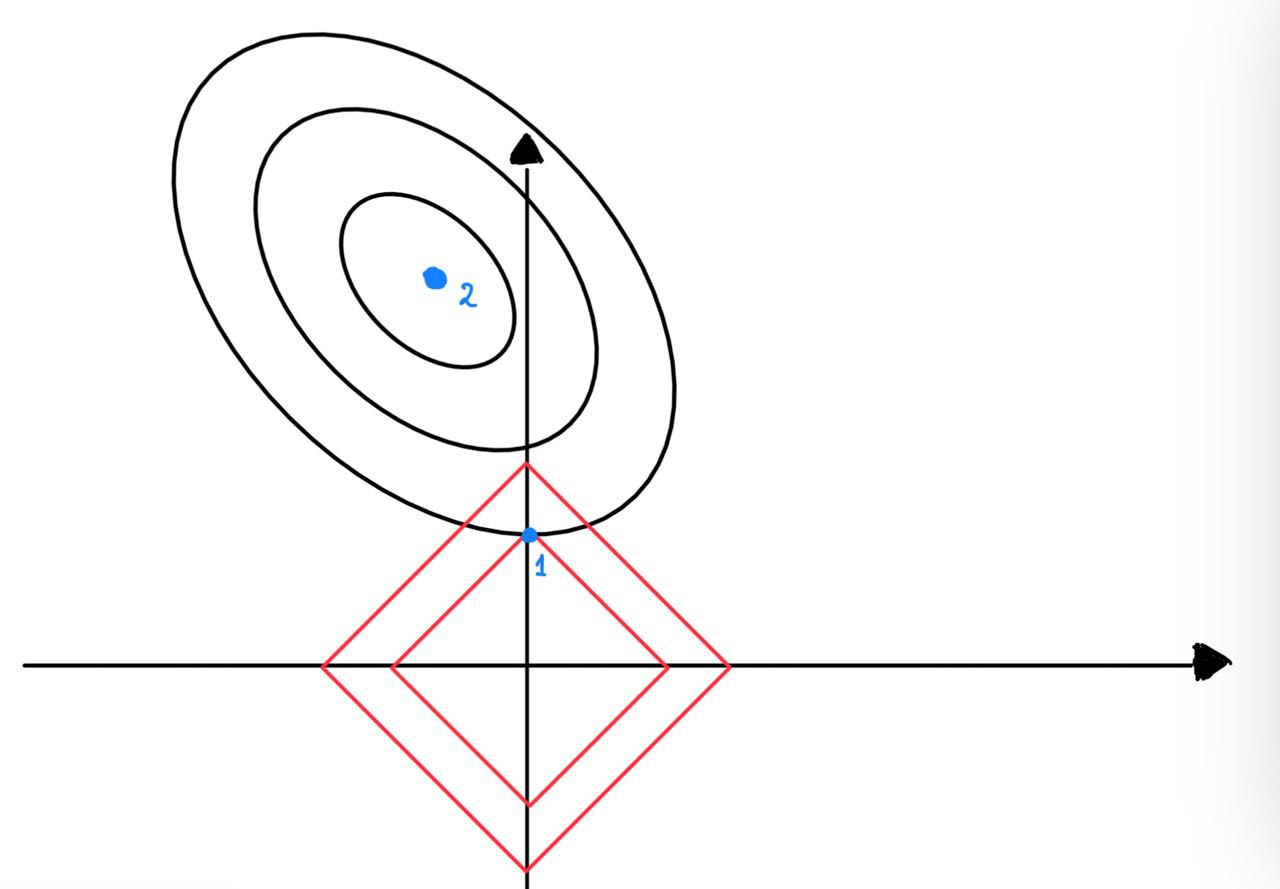
\includegraphics[trim=0cm 0cm 1.5cm 0cm, clip, width=0.5\textwidth]{photos/L1.jpg}
    \end{center}


    \subsection{Линейная классификация}


    \subsubsection{Разделяющий подход (SVM)}
    Во-первых, далее классы принадлежат множеству $\{-1, \ 1 \}$, пока не указано иное. В данной ситуации мы 
    пытемся найти разделяющую плоскость, которая будет делить пространство на два класса. 
    Есть две ситуации: 
    
    \begin{itemize}
        \item \textbf{Выборка линейно разделима}. В данном случае существует плоскость, которая идеально 
        разделит исходные данные на два класса, так что с одной стороны плоскости будут только самплы одного 
        класса, а с другой - другого 
        \item \textbf{Выборка не линейно разделима}. В данном случае такой гиперплоскости не существует
    \end{itemize}

    Итоговое предсказание может быть задано как 

    \begin{equation}
        y = \operatorname{sign}( \langle w, X_{i} \rangle)
    \end{equation}

    \quad 

    \quad

    Рассмотрим как работает классификация в целом, пусть задана решающая плоскость:

    \begin{equation}
        \langle w, x \rangle + b = 0
    \end{equation}

    (В нашем случае все точно также, только 1 в конце вшита в $X_{i}$, а $b$ в $w$). $w$ перпендикулярна 
    заданной плоскости. Это легко показать так: получим вектор лежащий на плоскости, для этого рассмотрим 
    две точки $x_{1}$ и $x_{2}$ обе из которых лежат на плоскости i.e  

    \[
    \begin{cases}
        \langle w, x_{1} \rangle + b = 0 \\ 
        \langle w, x_{2} \rangle + b = 0
    \end{cases}
    \]

    Рассмотрим вектор $x^{*} = x_{1} - x_{2}$, заметим, что данный вектор лежит на плоскости, 
    мы можем проверить его перпендикулярность $w$.

    \begin{equation}
        \langle w, x^{*} \rangle = \langle w, x_{1} - x_{2} \rangle = \langle w, x_{1} \rangle - \langle w, x_{2} \rangle = -b - (-b) = 0 
    \end{equation}

    Заметим, что $w^{*}$ соответствует любому вектору лежащему на плоскости, следовательно $w$ параллельна всей 
    плоскости. Рассмотрим геометрический смысл $\langle w, x \rangle + b$, где $x$ --- произвольный вектор, в нашей регрессии 
    это просто $\langle w, x \rangle$ для удобства. Мы знаем, что $w$ перепендикулярен плоскости
    т.е мы можем провести из произвольной точки $x$ перпендикулрную к плоскости прямую, используя $w$.
    $x_{new} = x + a w$, где $a$ --- произвольный коэффициент. При этом для $x_{new}$ выполняется 
    $\langle w, x_{new} \rangle + b = 0$. Найдем коэффициент $a$.

    \begin{equation}
        \langle w, x + a w \rangle + b = 0 
    \end{equation}

    Это равносильно

    \begin{equation}
        \langle w, x \rangle + a \langle w, w \rangle + b = 0
    \end{equation}

    Следовательно 

    \begin{equation}
        a = - \frac{\langle w, x \rangle + b}{\langle w, w \rangle}
    \end{equation}

    Нас интересует расстояние от $x$, до этой новой полученной точки, которое равно 

    \begin{equation}
        |a| \cdot \Vert w \Vert = |\frac{\langle w, x \rangle + b}{\Vert w \Vert^{2}}| \cdot \Vert w \Vert
    \end{equation}

    Следовательно искомое расстояние раввно

    \begin{equation}
        \frac{|\langle w, x \rangle + b|}{\Vert w \Vert}
    \end{equation}

    Получается мы имеем дело с числителем расстояния. 
    Заметим, что максимизация расстояния равносильна 
    
    \[
    \begin{cases}
        |\langle w, x \rangle + b| \rightarrow \max \\ 
        \Vert w \Vert \rightarrow \min 
    \end{cases}
    \]

    Мы воспользуемся этим далее 


    \quad

    \quad


    Продолжим. Мы хотим, чтобы 

    \begin{equation}
        \sum_{i} \text{I}[y_{i} \neq \operatorname{sign}( \langle w, X_{i} \rangle)] \rightarrow \min
    \end{equation}

    Или же 

    \begin{equation}
        \sum_{i} \text{I}[y_{i} \cdot \langle w, X_{i} \rangle < 0] \rightarrow \min
    \end{equation}

    Обозначии $\text{M} = y_{i} \cdot \langle w, X_{i} \rangle$, это называется отступом (margin) классификатора. 
    Можно легко заметить, что чем больше margin, тем лучше решается задача классификации. 
    Отступ положителен, когда $\text{I}[y_{i} = \operatorname{sign}( \langle w, X_{i} \rangle)]$, 
    то есть класс угадан верно, при этом чем больше отступ, тем больше расстояние от сампла
    до разделяющей гиперплоскости, то есть «уверенность классификатора».
    Таким же образом, если отступ отрицателен, то класс угадан неверно, 
    при этом, чем больше по модулю отступ, тем более сокрушительно ошибается классификатор.
    Нам нужно аппроксимировать индикатор непрерывной функцией

    Варианты аппроксимации: 

    \begin{center}
        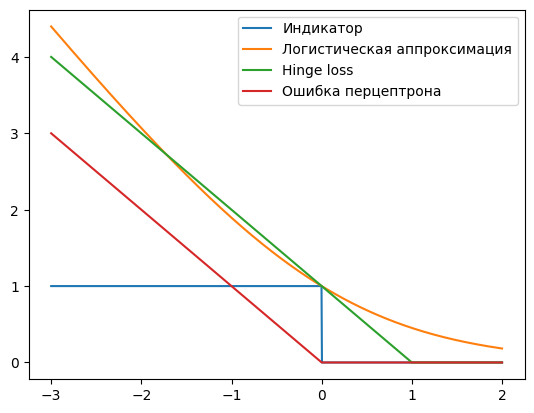
\includegraphics[width=0.5\textwidth]{photos/lin_mod_class_loss.png}
    \end{center}

    Распишем все представленные варианты

    \begin{itemize}
        \item \textbf{Логистическая}. Задается формулой $\log(1 + e^{-M})$, в примере делилась на $\log(2)$, чтобы 
        проходить через точку $(0, 1)$, но это не необходимо для задачи оптимизации
        \item \textbf{Ошибка перцептрона}. Задается как $\max(0, -M)$
        \item \textbf{Hinge loss}. Задается как $\max(0, 1 - M)$
    \end{itemize}

    Можно заметить, что последние два лосса очень похожи. Их разница лишь в том, что Hinge loss продолжает 
    штрафовать даже правильно классифицированные точки, если они приближаются к разделяющей плоскости слишком 
    близко, а именно если они находятся на расстоянии $\frac{1}{\Vert w \Vert}$ и ближе от разделяющей плоскости. 
    Итоговый функционал потерь задается как: 

    \begin{equation}
        \sum_{i} \text{loss}(y_{i}, X_{i}) + \lambda \Vert w \Vert^{2}
    \end{equation}
    
    На выходе мы получаем строго выпуклую функцию, что гарантирует уникальность найденного минимума.
    Это достигается за счет того, что норма --- строго выпуклая функция, а все три перечисленных выше 
    аппроксимации функции потерь
    являются выпуклыми, а сумма выпуклой и строго выпуклой функции дает строго выпуклую функцию.

    Как мы видим, данная задача оптимизации эквивалентна задаче

    \[
        \begin{cases}
            |\langle w, x \rangle + b| \rightarrow \max \quad (\text{При определенных условиях})\\ 
            \Vert w \Vert \rightarrow \min 
        \end{cases}
    \]

    Именно поэтому мы можем использовать $\langle w, x \rangle$ вместо расстояния до решающей плоскости при 
    оптимизации. Вот цитата из учебника ШАДа об SVM: 

    \begin{quote}
        Итоговое положение плоскости задаётся всего несколькими обучающими примерами. 
        Это ближайшие к плоскости правильно классифицированные объекты, 
        которые называют опорными векторами или support vectors. 
        Весь метод, соответственно, зовётся методом опорных векторов, 
        или support vector machine, или сокращённо SVM. 
        Начиная с шестидесятых годов это был сильнейший из известных методов машинного обучения. 
        В девяностые его сменили методы, основанные на деревьях решений.
        Почему же SVM был столь популярен? 
        Из-за небольшого количества параметров и доказуемой оптимальности. 
        Сейчас для нас нормально выбирать специальный алгоритм под задачу и подбирать 
        оптимальные гиперпараметры для этого алгоритма перебором, 
        а когда-то трава была зеленее, а компьютеры медленнее, 
        и такой роскоши у людей не было. 
        Поэтому им нужны были модели, которые гарантированно неплохо работали бы в любой ситуации. 
        Такой моделью и был SVM.
        Другие замечательные свойства SVM: существование уникального решения и 
        доказуемо минимальная склонность к переобучению среди всех популярных классов 
        линейных классификаторов. 
        Кроме того, несложная модификация алгоритма, ядровый SVM, 
        позволяет проводить нелинейные разделяющие поверхности.
    \end{quote}


    \subsubsection{Kernel-ы в SVM}

    \paragraph{Интуиция}

    \quad 

    Пусть в нашем пространстве данные не являются линейно разделимыми или они трудноразделимы.
    Мы хотим отобразить наши данные в новое пространство, где будем искать разделяющую плоскость.
    Мы предполагаем, что в этом новом пространстве использование разделяющей плоскости
    будет более эффективно, чем в исходном.
    Однако напрямую отображать данные в необходимое пространство вычислительно трудно,
    так же как и считать скалярное произведение между ними в нём. Однако мы можем 
    вычислить скалярное произвдение в целевом пространстве не переходя в него,это так называемый kernel trick.
    Вместо использования обычного скалярного произведения, мы используем kernel, который возвращает скалярное
    произведение репрезентаций двух переданных векторов в новом пространстве. Таким образом мы можем улавливать нелинейные 
    зависимости работая при этом в исходном пространстве. 

    \quad 

    (Cooming soon)

    \quad

    \subsubsection{Вероятностный подход}



    \section{Эмбеддеры в Word2Vec}
    Цель эмбедера - отобразить некий нечисловой объект в многомерное числовое пространство, так чтобы похожие 
    объекты в старом пространстве получали как можно более сонаправленные вектора в новом. 

    Существует два основных подхода к созданию эмбедеров в контексте Word2Vec, это 
    \begin{itemize}
        \item CBOW --- предсказывает слово по контексту. 
        Она работает быстрее, но, в силу своей логики, хуже улавливает семантику редких слов.
        \item Skip-Gram --- предсказывает контекст по слову. 
        Из-за необходимости обрабатывать несколько выходов для каждого слова 
        эта архитектура работает медленнее, зато лучше захватывает семантику редких слов.  
    \end{itemize}
    
    \paragraph*{Примечание}  
    Обе архитектуры основаны на концепции Bag of Words, которая утверждает, что 
    вся информация содержится в совокупности слов без учёта их порядка. Это справедливо только для небольших окон (эмпирическое наблюдение). Проявление 
    данной концепции можно будет наблюдать в использемых функциях потерь

    Обе архитектуры изначально использовали softmax выходной слой для предсказния вероятности по всем словам и log-loss 
    функцию потерь, предсказывая вероятности по всем словам словаря, однако более эффективным способом является Negative Sampling, 
    который является надстройкой над оргинальной моделью

    \subsection{CBOW}  
    Пусть в словаре \( n \) слов, каждое из которых имеет векторное представление. Рассмотрим множество окон \( K \), полученных из текстового корпуса. Каждое окно соответствует целевому слову \( w_{target} \). Для каждого \( k \in K \) мы стремимся максимизировать:  
    
    \[
    P(w_{target} \mid w_{context}) \rightarrow \max
    \]  
    
    Здесь \( w_{context} \) определяется как \( \text{mean}_{w \in k}(w) \). Этот вектор аккумулирует информацию о контексте.  
    
    Вероятность \( P(w_m \mid w_{context}) \) наблюдать слово \( w_m \) в контексте слов из \( w_{context} \) вычисляется как \( \sigma(w_{target} \cdot w_{context}) \).  
    
    Однако, мы не можем использовать такую функцию потерь, так как модель будет просто пытаться сделать векторы слова и контекста сонаправленными для каждого окна. 
    К функции максимизации добавляются потери на случайных словах, не входящих в текущее окно контекста, это и есть Negative Sampling. Мы минимизируем вероятность для таких слов, что приводит к итоговой формуле:  
    
    \[
    P(w_{target} \mid w_{context}) - \prod_{w_{rand} \notin k \mid w_{rand} \neq w_{target}} P(w_{rand} \mid w_{context}) \rightarrow \max
    \]  
    
    Это грубая аппроксимация log-loss функции, учитывающей все слова словаря в оригинальной реализации.  
    
    С точки зрения оптимизации, формула эквивалентна:  
    
    \[
    \log(P(w_{target} \mid w_{context})) + \sum_{w_{rand} \notin k \mid w_{rand} \neq w_{target}} \log(P(w_{rand} \mid -w_{context})) \rightarrow \max
    \]  
    
    CBOW использует две матрицы: одна кодирует контекст, другая — целевое слово и негативные примеры. Это реализует принцип разделения ответственности:  
    матрица контекста учится понимать контекст слова, а матрица целевых слов учится отражать семантику.  
    Обоснование использования двух матриц можно найти в статьях по теме:  
    
    \begin{quote}  
    Предполагается, что слова и контексты принадлежат разным словарям. 
    Например, вектор слова "собака" отличается от вектора контекста "собака". 
    Это связано с тем, что слова редко встречаются в своих собственных контекстах, 
    следовательно модель должна присваивать 
    низкую вероятность \( P(\text{собака} \mid \text{собака}) \), что требует 
    малой величины \( w_{собака} \cdot w_{собака} \). В оптимуме \( \|w_{собака}\| \rightarrow 0 \), что неправильно.  
    \end{quote}  

    Эта проблема скорее относится к оригинальной реализации. Negative Sampling частично решает данную проблему, так как минимизация вероятности выплняется не по всем словам вне окна, а по случайным словам, не 
    входящим в окно, также нужно учитывать, что при семплировании мы не берем целевое слово, что положительно сказывается на решении данной проблемы
    
    \subsection{Skip-Gram}  
    Логика этой модели похожа на CBOW, 
    но с несколькими ключевыми отличиями. 
    Мы работаем с вероятностями \( P(w_{context} \mid w_{target}) \), где \( w_{context} \) — множество векторов контекста.
    С добавлением негативного семплирования задача оптимизации принимает вид:  
    
    \[
    \sum_{w_i \in k} \log(P(w_i \mid w_{target})) + \sum_{w_{rand} \notin k \mid w_{rand} \neq w_{target}} \log(P(w_{rand} \mid -w_{target})) \rightarrow \max
    \]  
    
    В Skip-Gram используется одна матрица для всех векторов. Это связано с тем, что эмбеддинг должен аккумулировать информацию о контексте: предсказание вероятности контекста следует непосредственно из вектора слова.
    Проблема описанная выше, которая обосновывает использование двух матриц, решается с помощью Negative Sampling, который не позволяет минимизировать $\Vert w \Vert$

    \subsection{Выравнивание эмбеддингов}

    Допустим мы используем эмбеддеры для перевода слов с одного языка на другой. У нас могут быть размечены слова переводы для различных слов. 
    Мы хотим отобразить наши вектора в единое вектороное пространство, чтобы семантически похожие слова внутри разных языков 
    имели как можно более сонаправленные вектора в этом новом пространстве, так как это работает внутри одного языка. Есть два основных способа:

    \begin{itemize}
        \item MUSE (Multilingual Unsupervised and Supervised Embeddings)
        \item VecMap
    \end{itemize}

    Пусть у нас есть два словаря для двух разных языков $W_{c}$ --- словарь нашего языка, а $W_{f}$ --- словарь иностранных слов. 
    Формально можно считать, что существует два линейных пространства: $L_{c}$, $L_{f}$, таких, что 
    $\forall w_{c} \in W_{c} : w_{c} \in L_{c}$ и $\forall w_{f} \in W_{f} : w_{f} \in L_{f}$.
    Т.е каждый словарь опредлен над $L_{c}$ и $L_{f}$ соответственно. Цель выравнивания можно определить как 
    $L_{c} \rightarrow L_{f}$.

    Нам нужно привести словари к единому виду, так как они обучены на разных корпусах. Можно использовать общее подмножество слов.
    Например через явный перевод, или нахождение общих слов, таких как заимствованные. Мы создаем перекресный словарь по ним.
    Некоторые методы концентрируются на распределении векторов, не используя перекрестный словаь.
    
    \subsubsection{MUSE}

    Вот статья: https://arxiv.org/abs/1710.04087

    Исходя из названия поддерживает как supervised так и unsupervised режимы 

    \paragraph{Unsupervised}

    \quad

    Мы используем GAN для того, чтобы получить вектора с таким же распределением как и в целевом словаре.
    Однако в данном случае в качестве генератора выступает обыкновенная ортогональная матрица, 
    которая учится обманывать дискриминатор.
    При этом пары ``Слово-Перевод`` семплируются случайно, без смыслового сопоставления, так  
    как наша цель --- именно имитация распределения. Авторы оригинальной статьи использовали 50 тысяч
    самых часто встречающихся слов для обучения генератора для словарей размерами по 200 тысяч.
    Однако использование всех слов не приводило к значимому ухудшению результатов. 
    Слова выбирались равномерно, так как семплирование пропорционально частоте не дало улучшений.
    После того как мы обучили GAN, мы приступаем к Procrustes analysis (анализ Прокруста), предварительно 
    применив полученную матрицу ко всем эмбэддингам.

    \quad

    Рассмотрим задачу более подробно: 
    
    Наша цель --- найти такую матрицу $W$, что 

    \[
    \begin{cases}
        \Vert WX - Y \Vert_{F}^{2} \rightarrow \min \\
        W W^{T} = E \\
        W^{T} W = E
    \end{cases}
    \]

    Аналитически задача решается так: 

    Нам дано $\operatorname{trace}( ( WX - Y)^{T} (WX - Y))$, расскроем транспонирование и получаем 
    $\operatorname{trace}( ( X^{T} W^{T} - Y^{T}) (WX - Y)) = \operatorname{trace}( X^{T} W^{T} WX - X^{T} W^{T} Y   - Y^{T} WX + Y^{T} Y)$. 
    Так как $W^{T} W = E$. Расскроем выражение $\operatorname{trace}( X^{T}X - X^{T} W^{T} Y   - Y^{T} WX + Y^{T} Y)$. Так как 
    оптимизация выполняется по $W$, это равносильно $\operatorname{trace}(-X^{T} W^{T} Y   - Y^{T} WX)$. Следовательно

    \[
    \begin{cases}
        \operatorname{trace}(-X^{T} W^{T} Y   - Y^{T} WX) \rightarrow \min \\
        W W^{T} = E \\
        W^{T} W = E
    \end{cases}
    \]

    Мы можем преобразовать $\operatorname{trace}(-X^{T} W^{T} Y   - Y^{T} WX) \rightarrow \min$ в 
    $\operatorname{trace}(X^{T} W^{T} Y  + Y^{T} WX) \rightarrow \max$. Так как $\operatorname{trace}(A) = \operatorname{trace}(A^{T})$.
    Вся задача оптимизации сводится к $\operatorname{trace}(Y^{T} WX) \rightarrow \max$. Это можно свести к $\operatorname{trace}(WXY^{T}) \rightarrow \max$.
    Пусть $M = XY^{T}$. Тогда нам нужно оптмизировать $\operatorname{trace}(WM)$. По теореме Eckart–Young–Mirsky, максимум будет достигаться 
    в $W=UV^{T}$

    \quad

    Вот как происходит обучение в рамках Procrustes analysis:
    Во-первых, мы выбираем наиболее частые слова для данного этапа. Во-вторых, мы образуем синтетический словарь, на основе
    Cross-Domain Similarity Local Scaling (CSLS). Обсудим это подробнее: 


    \subparagraph{CSLS}

    \quad

    Мы не можем просто использовать NN, так как с таким подходом часто возникает ситуация, что для пары
    $(x, y)$, где $y$ --- ближайший к $x$ вектор, далеко не всегда выполняется, что $x$ -- ближайший к $y$ вектор.
    Авторы ссылаются на статью, которая показывает, что в высокоразмерных пространствах это приводит к образованию ``хабов``
    и ``антихабов`` --- векторов, которые являются соседями сразу для многих или не практически не являются соседями ни для кого,
    соответственно. Для решения данной проблемы мы бдуем ``штрафовать`` точки за то, что они являются хабами.
    Пусть мы будем использовать для этого $K$ соседей.
    Определим пару функций: $N_{c'}(x)$ --- функция, которая возвращает первые $K$ соседей вектора $x$ из словаря 
    $W_{c}'$, который образован путем применения генератора ко всем эмбеддингам из $W_{c}$. Аналогичная функция для $W_{f}$
    --- $N_{f}(x)$. Определим еще две функции: 

    \begin{equation}
        r_{c'}(x) = \frac{1}{K} \sum_{y \in N_{c'}(x)} cos(x, y)
    \end{equation}
    где $cos$ --- косинусная метрика. Также введем аналогчиную функцию для $W_{f}$ --- $r_{f'}(x)$.

    Введем финальную функцию: 

    \begin{equation}
        \text{CSLS}(x, y) = 2 \cdot cos(x, y) - r_{c'}(y) - r_{f}(x)
    \end{equation}
    где $x \in W_{c'}$ и $y \in W_{f}$

    Получается для каждого языка мы ищем соседей в противоположном. Такая фнукция сходства штрафует векторы, которые 
    лежат в плотных областях. И по наблюдениям авторов метода использование CSLS дает значительное улучшение показателей.
    
    \quad 

    Мы создаем синтетический словарь, ищя MNN (Mutal Nearest Neigh.) по CSLS на каждой итерации.
    Далее, для этого словаря мы ищем матрицу $W$ по алгоритму выше и применяем ко всем эмбэддингам. 
    Процесс повторяется итерационно. Согласно эмпирическим данным, обычно хватает от 5 до 10 итераций.
    Итоговая функция для трансформации вектора в новое пространство имеет вид 

    \begin{equation}
        \prod_{i = 0}^{n - 1} W_{n - i} \cdot W_{G} \cdot x
    \end{equation}
    где $W_{G}$ - матрица генератора

    \paragraph{Supervised}

    \quad

    Если у нас есть перекрестный словарь, то мы переходим сразу к шагу Procrustes анализа. Однако нужно учитывать, что, несмотря 
    на название, метод разрабатывался для unsupervised режима работы

    \subsubsection{VecMap}

    В первую очередь мы нормализуем эмбэддинги, а также центрируем каждую координату. После этого мы снова применяем 
    нормализацию. Пострим матрицы $M_{X} = X^{T} X$ и $M_{Y} = Y^{T}Y$ (тут предполагается, что $X$ и $Y$ --- словари в которые по столбцам записаны эмбэддинги).
    Если пространства эмбэддингов полностью изометричны, то существует такая перестановка строк или столбцов что матрицы $M_{X}$ и $M_{Y}$ будут равны.
    Тут предполагается, что размеры словарей по которым будет производиться выравнивание равны, также как и размерности эмбеддингов. 
    На практике изометрия выполняется приближённо, а поиск перестановок NP-полная задача. 

    Возьмем и независимо отсортируем каждую строку в $M_{X}$ и в $M_{Y}$, получив матрицы $\text{sorted}(M_{X})$
    и $\text{sorted}(M_{Y})$. 
    При условии идеальной изометрии получившиеся матрицы 
    будут равны с точностью до перестановки строк. Исходя из предположения, что изометрия приближенно выполняется
    мы можем искать ближайших соседей для строки из одной матрицы среди строк другой матрицы и считать, что найденный ближайший сосед 
    является репрезентацией исходной строки в другом пространстве. 

    Важное замечание: если мы используем SVD для матриц эбэддингов (т.е $X = U \Sigma V^{T}$) 
    то получим, что $M_{X} = V \Sigma U^{T}  U \Sigma V^{T} = V \Sigma^{2} V^{T}$. Авторы оригинальной 
    статьи заметили, что использование матрицы $\sqrt{M_{X}} = V \Sigma V^{T}$ более эффективно 
    (в оригинале использовалась матрица $U \Sigma U^{T}$, так как эмбеддинги были записаны по строкам).

    Процесс обучения мы начинаем с формирования небольшого словаря, например 25 слов. Для его формирования мы используем алгоритм описанный выше 
    (в оригинальной статье использовались 4000 наиболее частых слов для создания начального словаря). 
    Далее по известному алгоритму из Procrustes анализа находим 
    ортгональную матрицу $W$, используя только эмбеддинги из словаря, которую после применяем ко всем эмбеддингам. 
    Далее мы пытаемся добавить новое слово 
    в словарь, для этого мы используем алгоритм из начала. 
    Для этого мы ищем ближайшего соседа для каждой строки из корня sorted версии матрицы схожести 
    одного языка в такой же матрице другого языка, пару наиболее похожих слов мы добавляем в словарь. 
    После снова переходим к поиску матрицы $W$, итеративно повторяя весь процесс с новым словарем.

    Однако такой сырой алгоритм нуждается в дополнениях. Вот некоторые из них: 

    \begin{itemize}
        \item Dropout. Для каждого вектора при поиске его соседей, каждый сосед с вероятностью 
        $1 - p$ игнорируется, т.е мы зануляем веса связи с вероятностью $1 - p$. В предложенной авторами метода
        реализации мы начинаем с $p = 0.1$ (сильный стохастический шум). Если целевая функция не улучшается 50 итераций подряд, 
        увеличиваем $p$ в 2 раза (аналог simulated annealing). 
        \item Использование наиболее частых слов. Для обучения мы используем лишь первые 
        20000 наиболее частых слов в каждом языке.
        \item MNN + CSLS. Как и в MUSE, для поиска нового слова мы используем MNN + CSLS, вместо обычного NN.
    \end{itemize}

    \section{Контекстуальные эмбэддеры} 

    \textbf{
        Нужно заметить, что сейчас статические эмбэддеры 
        не используются, так как на рынке доминируют контекстуальные эмбэддеры,
        т.е вектор слова меняется в зависимости от контекста в котором оно находится
    }

    \quad  

    Примеры контекстуальных эмбэддеров:
    \begin{itemize}
        \item \textbf{ELMo}. Использует двунаправленные LSTM 
        \item \textbf{BERT}. Использует трансформеры и учится на задачах маскирования.
        Маскирование похоже на CBOW, часть слов в окне маскируется и заменяется на токен маски.
        После этого модель пытается предсказать на основе контекста, что за слово скрыто за токеном маски.  
    \end{itemize} 

    (Информация по ним будет внесена позже)


    \section{ONNX}

    ONNX (Open Neural Network Exchange) - формат для представления моделей из разных фреймворков в унифицированном виде.
    Это позволяет передавать модели между ними, а также ONNX удобен для инференса 








\end{document}